\documentclass[12pt]{beamer}

\usetheme[progressbar=frametitle]{metropolis}
\usepackage{appendixnumberbeamer}
\usepackage{subcaption}
\usepackage{siunitx}

\newcommand{\pder}[2]{\frac{\partial#1}{\partial#2}}
\newcommand{\pdder}[2]{\frac{\partial^2#1}{\partial#2^2}}
\newcommand{\myabs}[1]{\vert#1\vert}

\DeclareMathOperator{\iso}{Iso}
\DeclareMathOperator{\fix}{Fix}
\DeclareMathOperator{\tr}{Tr}
\DeclareMathOperator{\vol}{vol}


\title{Hearing the Local Orientability of Orbifolds}
% \date{\today}
\date{}
\author{Sean Richardson '20, Liz Stanhope}
\institute{Department of Mathematical Sciences, Lewis \& Clark College}

\begin{document}

\maketitle

\begin{frame}{Listening to Drums}
    \begin{itemize}
        \item If you have a drum, the sound the drum makes is determined
        \item<2-> However, if you hear a drum being played in another room, what can you
            say about it?
        \item<3-> Can you hear the shape of a drum?
        \item<4> Can you hear the shape of mathematical objects called
            ``orbifolds''?
    \end{itemize}
\end{frame}

\section{What is an Orbifold?}



\begin{frame}{Reflectional Symmetry}
    \begin{itemize}
        \item We classify symmetries with the group of isometries that
            leave a pattern unchanged
        \item Figure~\ref{fig:ref_sym} has group $\Gamma = \{ e, r \} $
        \item One line in space is left unmoved by all $g \in \Gamma$.
        \item We can fold the space into $\mathbb{R}^2/\Gamma$
    \end{itemize}
    \begin{columns}
        \begin{column}[c]{0.39\textwidth}
    \begin{figure}
    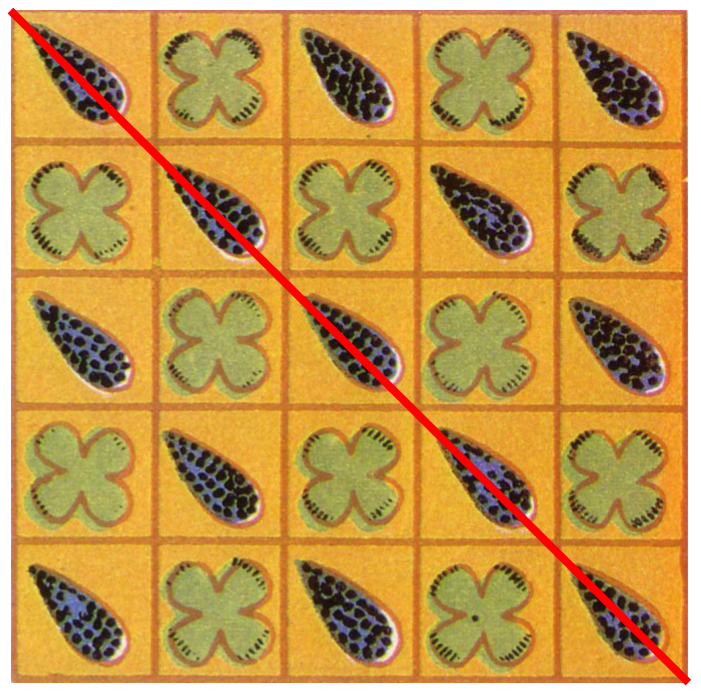
\includegraphics[width=0.7\textwidth]{images/reflection_with_line.png}
    \caption{Reflectional Symmetry}
    \label{fig:ref_sym}
    \end{figure}
    \end{column}
    \begin{column}[c]{0.49\textwidth}
    \begin{figure}
    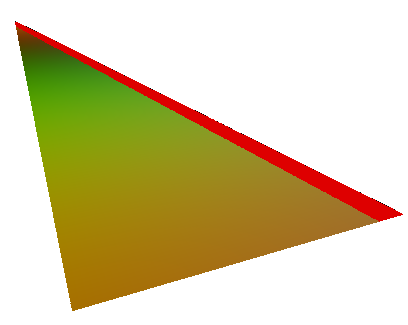
\includegraphics[width=0.6\textwidth]{images/mirror_edge.png}
    \caption{Folding the Pattern}
    \end{figure}
    \end{column}
    \end{columns}
\end{frame}

\begin{frame}{Rotational Symmetry}
    \begin{itemize}
        \item We classify symmetries through the group of isometries that
            leave a pattern unchanged
        \item Figure~\ref{fig:rot_sym} has group $\Gamma = \{ \ang{0},
            \ang{90}, \ang{180}, \ang{270} \}$
        \item One point is left unmoved by all $g \in \Gamma$
        \item We can twist the space into $\mathbb{R}^n/\Gamma$ creating a
            party hat
    \end{itemize}
    \begin{columns}
        \begin{column}[c]{0.35\textwidth}
    \begin{figure}
    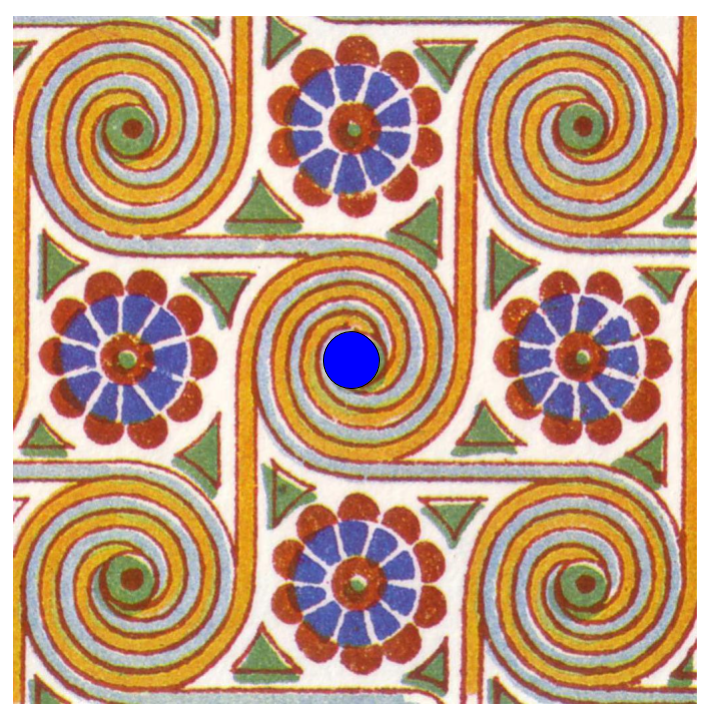
\includegraphics[width=0.7\textwidth]{images/rotation_with_dot.png}
    \caption{Rotational Symmetry}
    \label{fig:rot_sym}
    \end{figure}
    \end{column}
    \begin{column}[c]{0.3\textwidth}
    \begin{figure}
    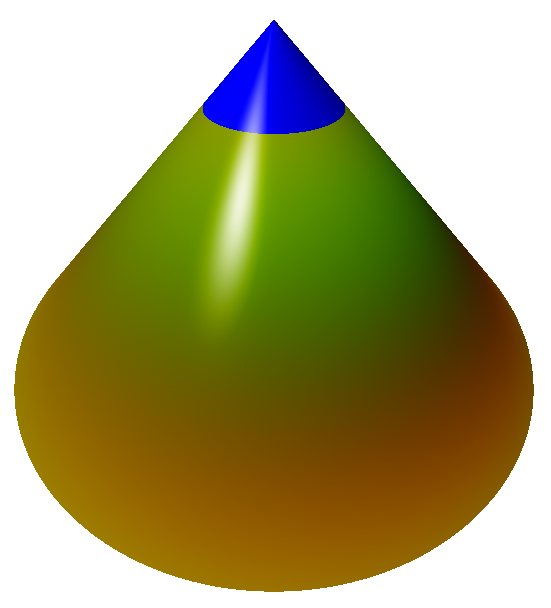
\includegraphics[width=0.8\textwidth]{images/cone_point.png}
    \caption{Folding the Pattern}
    \end{figure}
    \end{column}
    \end{columns}
\end{frame}



\begin{frame}{Orbit-folding}
    \begin{itemize}
    \item We fold a pattern such that no section occurs twice.
    \item Result has mirror edge and cone point strata.
    \end{itemize}
    \begin{figure}
    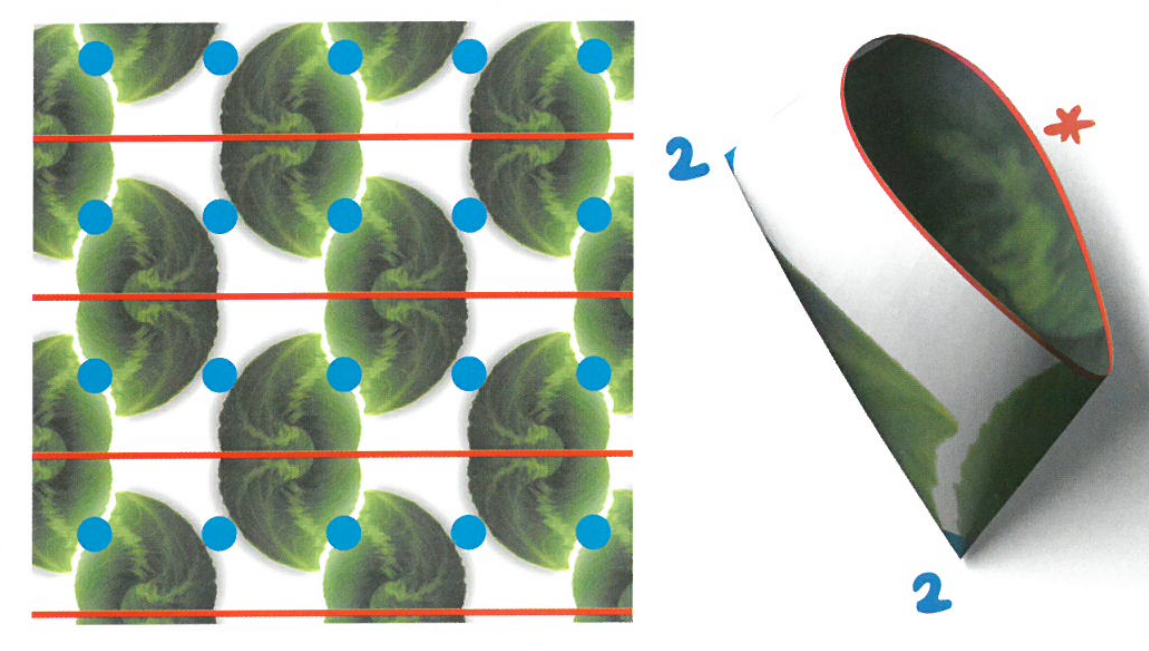
\includegraphics[width=0.6\textwidth]{images/wallpaper.png}
    \caption{Folded Pattern from \textit{The Symmetries of Things}}
    \end{figure}
\end{frame}
%Symmetries motivate orbifolds...

\begin{frame}{Orbifolds}
    \begin{columns}[c]
    \begin{column}[c]{0.5\textwidth}
    \begin{itemize}
        \item An \emph{orbifold} is a generalization of a manifold.
        \item While a manifold has local structure $\mathbb{R}^n$, an
            orbifold is allowed local structure $\mathbb{R}^n/\Gamma$
    \end{itemize}
\end{column}
\begin{column}[c]{0.49\textwidth}
    \begin{figure}
        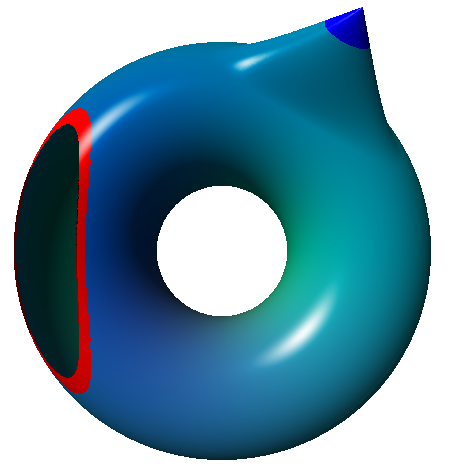
\includegraphics[width=\textwidth]{images/orbifold_ex.png}
        \caption{Orbifold Representation}
    \end{figure}
\end{column}
\end{columns}
\end{frame}

\section{What is the ``Sound'' of an Orbifold?}

\begin{frame}{Sound Comes from Vibration}
\begin{columns}[c]
\begin{column}[c]{0.49\textwidth}
    \begin{itemize}
        \item Like physical objects, the ``sound'' of an orbifold is defined by how quickly it
            vibrates.
    \end{itemize}
\end{column}
\begin{column}[c]{0.5\textwidth}
    \begin{figure}
    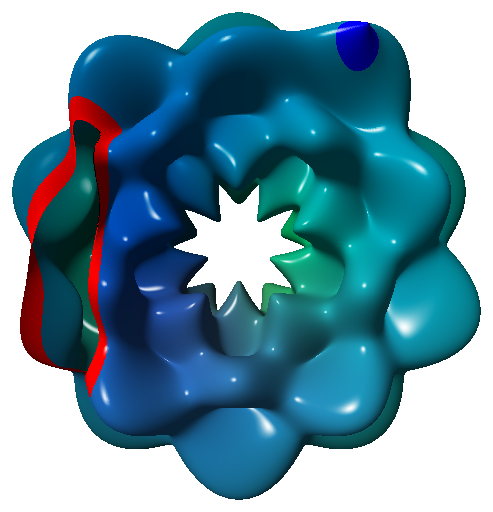
\includegraphics[width=\textwidth]{images/wavey_torus.png}
    \caption{Orbifold Vibration}
    \end{figure}
\end{column}
\end{columns}
\end{frame}


\begin{frame}{The Wave Equation}
   \begin{itemize}
       \item Let $u(t,\mathbf{x})$ be the amplitude of the wave at time $t$
           and position $\mathbf{x}$
       \item The orbifold will vibrate according to the wave equation,
           $$\Delta \psi = \pdder{u}{t}$$
       \item Assuming $u(t,\mathbf{x})=A(t)\psi(\mathbf{x})$ for standing
           wave solutions results in
           $$\Delta \psi(\mathbf{x}) = -\lambda \psi(\mathbf{x})$$
   \end{itemize}
\end{frame}

\begin{frame}{Laplace Spectra}
        $$\Delta \psi(\mathbf{x}) = -\lambda \psi(\mathbf{x})$$
    \begin{itemize}
       \item Eigenvalue solutions form a discrete spectrum $\lambda_1, \lambda_2,
           \lambda_3, \dots$ such that $\sqrt{\lambda_i}$ is a fundamental
           frequency. 
       \item This spectrum $\lambda_1, \lambda_2, \lambda_3, \dots$ is
           called the Laplace Spectra.
       \item The Laplace Spectra defines ``sound'' on an orbifold.
    \end{itemize}
\end{frame}
\begin{frame}{Research Question}
    \begin{itemize}
        \item ``Can you hear the shape of an orbifold?''
        \item \textbf{What properties of an unknown orbifold $\mathcal{O}$
            are determined by it's known Laplace Spectra?}
            \begin{itemize}
                \item Can you hear the types/amount of strata on an
                    orbifold?
                \item Can an orbifold and a manifold have the same Laplace
                    Spectra?
            \end{itemize}
    \end{itemize}

\end{frame}

\section{Heat Expansion}

\begin{frame}{Intuition of Heat Expansion}
    \begin{columns}[c]
        \begin{column}{0.46\textwidth}
    Consider:
    \begin{itemize}
        \item Heat up a point $\mathbf{x}$ on an orbifold $\mathcal{O}$
        \item Then, allow the heat to disperse
        \item The point cools down with time
    \end{itemize}
\end{column}
\begin{column}[c]{0.53\textwidth}
    \begin{figure}
        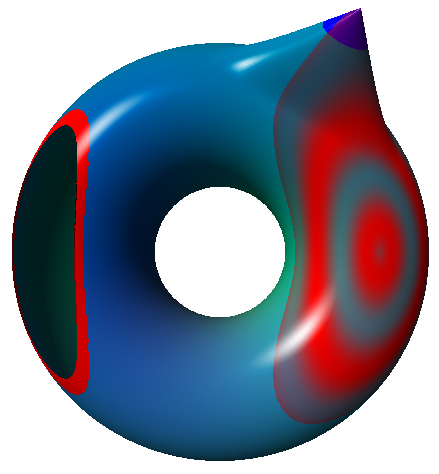
\includegraphics[width=\textwidth]{images/heat_ex.png}
        \caption{Heat Dispersing from $\mathbf{x}$}
    \end{figure}
\end{column}
\end{columns}
\end{frame}

\begin{frame}{Intuition of Heat Expansion}
    We study a specific function:
    \begin{itemize}
        \item How does a point cool with time on average for every point in
            the orbifold $\mathcal{O}$?
        \item We approximate this function for small values of time.
        \item This function is related to the Laplace Spectrum.
    \end{itemize}
\end{frame}

\begin{frame}{The Heat Equation}
    \begin{itemize}
    \item Let $u(t,\mathbf{x})$ be the heat at time $t$ and position
        $\mathbf{x}$ on an
        orbifold $\mathcal{O}$
    \item Heat will spread through $\mathcal{O}$ according to the heat
        equation
        $$\Delta u = \pder{u}{t}$$
    \item The solution to the heat equation has the form,
        $$u(t,\mathbf{x}) =
        \int_{M}K(t,\mathbf{x},\mathbf{y})\mu_0(y)dvolM_y$$
    \item Consider the function $K(t,\mathbf{x},\mathbf{y})$, the ``heat
        kernel''
    \end{itemize}
\end{frame}

\begin{frame}{Heat Kernel}
    \begin{itemize}
        \item If heat starts at $\mathbf{p}$, there is
            $K(t,\mathbf{p},\mathbf{q})$ heat at $\mathbf{q}$ at time $t$.
    \item Taking the trace of $K$ relates to the elements of the Laplace
        Spectra.
        $$\tr(K) = \int_{M}K(t,\mathbf{x},\mathbf{x})dvolM =
        \sum_{j=0}^{\infty} e^{-\lambda_j t}$$
    \end{itemize}
    \begin{figure}
        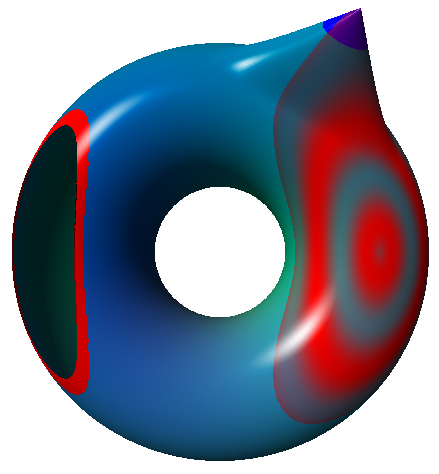
\includegraphics[width=0.25\textwidth]{images/heat_ex.png}
        \caption{Heat Dispersing from $\mathbf{p}$}
    \end{figure}
\end{frame}

\begin{frame}{Asymptotic Expansion of Heat Kernel}
    \begin{itemize}
    \item The Heat trace has a useful approximation for small values
        of time.
        $$\tr(K) \stackrel{t \to 0}{\sim}
        \frac{a}{t} + \frac{b}{\sqrt{t}} + c + d\sqrt{t} + et + \dots$$
    \item Because we now know $\tr(K) = \sum_{j} e^{-\lambda_j t}$,
        $$\sum_{j=0}^{\infty} e^{-\lambda_j t} \stackrel{t \to 0}{\sim} 
        \frac{a}{t} + \frac{b}{\sqrt{t}} + \dots$$
    \item A different value of any coefficient $a,b,c,\dots$ implies a
        different Laplace Spectra $\lambda_1, \lambda_2, \lambda_3, \dots$
    \end{itemize}
\end{frame}

\begin{frame}{Asymptotic Expansion of Heat Kernel}
    Meaning of  
        $\sum_{j=0}^{\infty} e^{-\lambda_j t} \stackrel{t \to 0}{\sim} 
        \frac{a}{t} + \frac{b}{\sqrt{t}} + \dots$ graphically:
    \begin{figure}
        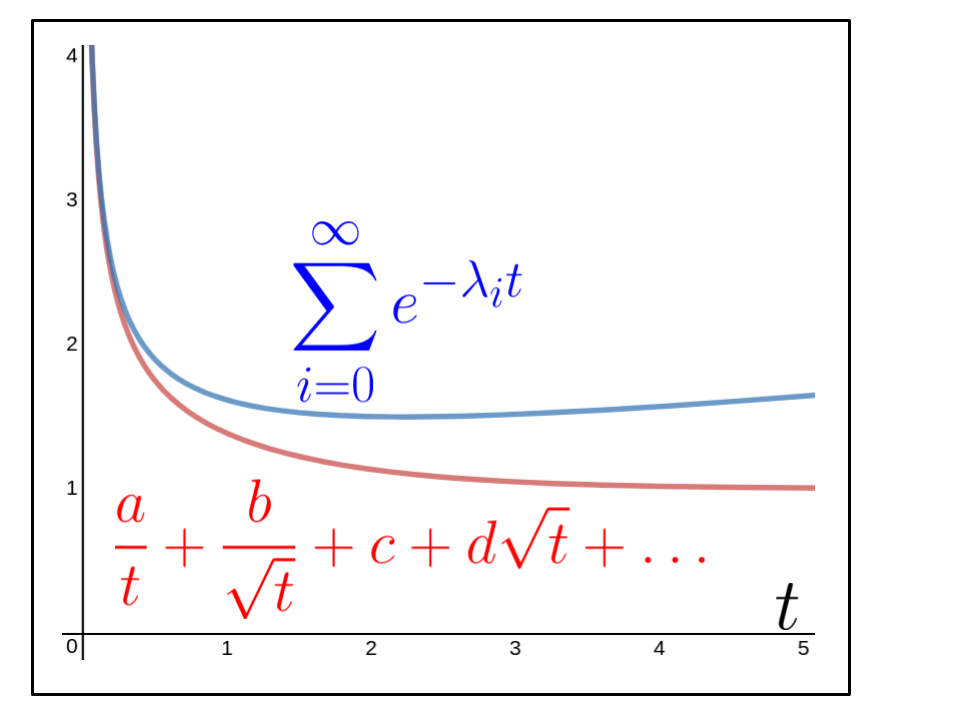
\includegraphics[width=0.5\textwidth]{images/heat_exp_graph2.png}
        \caption{Asymptotic Expansion Approximation}
    \end{figure}
\end{frame}

\begin{frame}{Heat Expansion Coefficients}
    We find the coefficients of the heat expansion through the following
    expression:
       \begin{align*}
           &{(4\pi t)}^{-\dim(\mathcal{O})/2}\sum_{k=0}^{\infty}a_k(\mathcal{O})t^k \\
            &+\sum_{N \in S(\mathcal{O})}\frac{{(4\pi t)}^{-\dim(N)/2}}{\myabs{\iso(N)}}\sum_{k=0}^{\infty}t^k\int_{N} \sum_{\gamma \in \iso^{\max}(\tilde{N})}b_k(\gamma,x) dvol_N
       \end{align*}
    Notes:
    \begin{itemize}
        \item The strata in the orbifold affect the expansion
        \item Even strata and odd strata behave differently
    \end{itemize}
\end{frame}

\section{Result}
\begin{frame}{Local Orientability}
    \begin{itemize}
        \item An isometry $g$ can preserve or reverse orientation
        \item<2-> The local structure $\mathbb{R}^n/\Gamma$ of some orbifold
            $\mathcal{O}$ is \emph{non-orientable} if $\Gamma$ contains a
            single orientation reversing isometry.
        \item<3-> We say $\mathcal{O}$ is \emph{locally non-orientable} if
            $\mathcal{O}$ contains some non-orientable local structure,
            otherwise $\mathcal{O}$ is \emph{orientable}.
        \item<4-> Local orientability can be interpreted through the
            existence of a short orientation reversing path.
    \end{itemize}
\end{frame}

\begin{frame}{We Can Hear Local Orientability}
    \begin{itemize}
        \item We found that you can hear the local orientability of an
            orbifold $\mathcal{O}$. 
        \item There exist no locally orientable orbifold and locally
            non-orientable orbifold with the same Laplace Spectra.
    \end{itemize}
    \begin{figure}
        \begin{columns}[c]
            \begin{column}[c]{0.28\textwidth}
                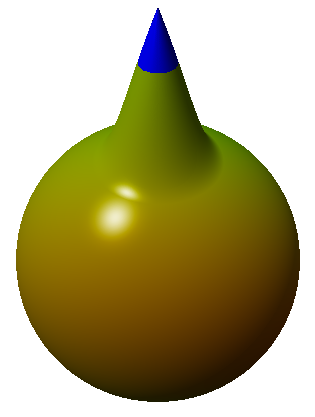
\includegraphics[width=\textwidth]{images/teardrop.png}
            \end{column}
            \begin{column}[c]{0.28\textwidth}
                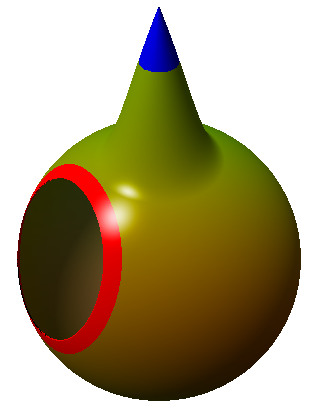
\includegraphics[width=\textwidth]{images/teardrop_edge.png}
            \end{column}
        \end{columns}
        \caption{Two Orbifolds with Different Laplace Spectra}
    \end{figure}
\end{frame}


\begin{frame}{Proof Framework}
    \begin{itemize}
        \item Let $\mathcal{O}_o$ be some locally orientable odd orbifold and
            let $\mathcal{O}_n$ be some locally non-orientable odd orbifold.
        \item $\mathcal{O}_o$ will have no even strata while
            $\mathcal{O}_n$ will have at least one even strata.
    \end{itemize}
\begin{center}
    \begin{table}
\begin{tabular}{c | c c c c c c c}
    & \dots & $t^{-1}$ & $t^{-1/2}$ & $t^{0}$ & $t^{1/2}$ & $t^{1}$ & \dots\\
\hline
$\mathcal{O}_o$ &
    \dots & $0$ & $\#$ & $0$ & $\# $& $0$ & \dots \\
$\mathcal{O}_n$ &
\dots & $d_{-1}$ & $\#$ & $d_0$ & $\# $& $d_1$ & \dots  \\
\end{tabular}
\caption{Heat expansion coefficients}
\end{table}
\end{center}

We are able to prove that at least one $d_i$ is non-zero. So,
$\mathcal{O}_o$ and $\mathcal{O}_n$ have distinct heat expansions, which
implies different Laplace Spectra.

\end{frame}

\section{Questions?}

\end{document}
